\documentclass[a4paper,12pt]{article}

\usepackage{tikz}
\usepackage{tabularx}
\usepackage{amsmath}
\usepackage[utf8]{inputenc}
\usepackage{multicol}
\usepackage{amsmath, amssymb, amsthm}
\usepackage{enumitem}
\usepackage{array}
\usepackage[left=2cm, right=2cm, top=2cm, bottom=2cm]{geometry}
\usepackage{fancyhdr}
\usepackage{xfp}
\usepackage{pgf}

\usepackage{graphicx}
\usepackage{fancyhdr}

\setlength{\headheight}{28pt}
\pagestyle{fancy}
\fancyhf{} % alles leeren

% Kopfzeile
\fancyhead[L]{\includegraphics[height=1.2cm]{logo.png}}
\fancyhead[C]{\small Beispielaufgaben-Klassenarbeit\\ Heinrich-von-Kleist-Schule}
\fancyhead[R]{\small Mathematik – G10B\\ Name:\ \rule{2.8cm}{0.4pt}}

% Fußzeile
\fancyfoot[C]{Seite \thepage \enspace\textbullet\enspace
	J.\,Mycan \textcopyright~2025\ *Klassenarbeit 45 min.*}

\renewcommand{\footrulewidth}{0.4pt}



\newcommand{\punkteA}{0}
\newcommand{\punkteB}{0}
\newcommand{\punkteC}{0}
\newcommand{\punkteD}{0}
\newcommand{\punkteE}{0}

\newcommand{\maxSumme}{45}
\newcommand{\noteEinsMin}{\fpeval{round(\maxSumme * 0.95,0)}}
\newcommand{\noteZweiMin}{\fpeval{round(\maxSumme * 0.80,0)}}
\newcommand{\noteDreiMin}{\fpeval{round(\maxSumme * 0.60,0)}}
\newcommand{\noteVierMin}{\fpeval{round(\maxSumme * 0.45,0)}}
\newcommand{\noteFunfMin}{\fpeval{round(\maxSumme * 0.20,0)}}
\newcommand{\noteSechsMin}{0}

\newcommand{\summe}{%
	\pgfmathparse{\punkteA + \punkteB + \punkteC + \punkteD + \punkteE}%
	\pgfmathprintnumber{\pgfmathresult}}

\begin{document}
	
%	\begin{center}
%		\textbf{Vorbereitung auf die Klassenarbeit - Potenzen}
%	\end{center}
	
	\textbf{Vor- und Nachname:} \underline{\hspace{10cm}}\\[0.1cm]
	Die Lösungen sowie Lösungswege sollten klar strukturiert und gut nachvollziehbar sein.\\[0.1cm]
	
\textbf{Aufgabe 1 (Punkte)}\\
Bei einem Experiment wird eine kleine Rakete senkrecht nach oben gestartet. 
Ihre Höhe über dem Boden (in Metern) in Abhängigkeit von der Zeit \(t\) (in Sekunden nach dem Start) 
kann näherungsweise durch die quadratische Funktion
\[
f(x) = -\frac{1}{100}x^2 + \frac{199}{200}x + \frac{1}{2}.
\]
beschrieben werden.

\begin{enumerate}
	
	\item[a)]
	Bestimme die Starthöhe der Rakete. Erläutere in einem Satz, was dieses Ergebnis im Sachzusammenhang bedeutet. 
	
	\item[b)]
	Bestimme, nach welcher Zeit die Rakete wieder den Boden erreicht. 
	Begründe, welchen der gefundenen Werte du im Sachzusammenhang verwendest. 
	
	\item[c)]
	Berechne, nach welcher Zeit die Rakete ihre maximale Höhe erreicht, und gib diese maximale Höhe an. 
	Formuliere die Bedeutung der beiden Werte im Sachzusammenhang.
\end{enumerate}

\textbf{Aufgabe 2 (Punkte)}\\
	Gegeben ist die Gerade \(g\) mit der Gleichung
	\[
	g:\; f(x) = x + 1
	\]
	sowie der Punkt \(Q(3\mid -1)\).
	
	\begin{enumerate}
		\item[a)] Fertige eine Skizze der Geraden \(g\) und des Punktes \(Q\) in ein Koordinatensystem an. 
		
		\item[b)] Bestimme den Punkt \(P\) auf der Geraden \(g\), der vom Punkt \(Q\) den kleinsten Abstand hat,
		und berechne diesen minimalen Abstand.
	\end{enumerate}

\textbf{Aufgabe 3 (Punkte))}\\
	Löse die folgenden Gleichungen. Vereinfache jeweils sinnvoll und gib alle Lösungen an.
	\begin{enumerate}
		\item[a)] \(2x^2 - 5x + 1 \;=\; x^2 + 4x - 2\)
		
		\item[b)] \((x - 3)^2 + 2x \;=\; 2x^2 - x + 5\)
		
		\item[c)] \(3(x+1)^2 - 4 \;=\; 2x^2 + x + 5\)
		
		\item[d)] \(2x(x-1) + 3 \;=\; (x-2)^2\)
	\end{enumerate}

\textbf{Aufgabe 4 (Punkte)}\\
Dem abgebildeten Dreieck ist ein Rechteck einbeschrieben. 
Das Rechteck liegt mit seiner unteren Seite auf der $x$-Achse, 
der rechte obere Eckpunkt hat die Koordinaten \(P(x_P\mid y_P)\).

\begin{center}
	\begin{tikzpicture}[scale=0.8]
		% Achsen
		\draw[->] (-2.5,0) -- (6.5,0) node[below right] {$x$};
		\draw[->] (0,-0.5) -- (0,4.5) node[left] {$y$};
		
		% Achsenbeschriftungen
		\draw (-2,0.1) -- (-2,-0.1) node[below=4pt] {$-2$};
		\draw (0,0.1) -- (0,-0.1) node[below=4pt] {$0$};
		\draw (6,0.1) -- (6,-0.1) node[below=4pt] {$6$};
		\draw (0.1,4) -- (-0.1,4) node[left=4pt] {$4$};
		
		% Dreieck
		\coordinate (A) at (-2,0);
		\coordinate (B) at (6,0);
		\coordinate (C) at (0,4);
		\draw[thick] (A) -- (C) -- (B) -- cycle;
		
		% Rechteck (Beispiellage, nur zur Veranschaulichung)
		\coordinate (R1) at (-1,0);
		\coordinate (R2) at (3,0);
		\coordinate (R3) at (3,2);
		\coordinate (R4) at (-1,2);
		\fill[green!30] (R1) -- (R2) -- (R3) -- (R4) -- cycle;
		\draw (R1) -- (R2) -- (R3) -- (R4) -- cycle;
		
		% Punkt P
		\fill (R3) circle (1.5pt);
		\node[above right] at (R3) {$P(x_P\mid y_P)$};
	\end{tikzpicture}
\end{center}

\noindent
Dem Dreieck soll ein Rechteck mit möglichst großem Flächeninhalt 
einbeschrieben werden.

\begin{enumerate}
	\item[a)] Fertige eine Skizze der Situation in dein Heft und übernimm die Bezeichnungen.
	\item[b)] Bestimme, wie der Punkt \(P\) gewählt werden muss, damit der Flächeninhalt
	des Rechtecks maximal wird, und berechne diesen maximalen Flächeninhalt.
\end{enumerate}

	\textbf{Aufgabe 5 (Punkte)}\\
	Löse die folgenden Potenzgleichungen. Vereinfache jeweils sinnvoll und gib alle Lösungen an.

	\begin{enumerate}
	\item[a)] \(2^{x+1} + 8 \;=\; 4\cdot 2^{x}\)
	
	\item[b)] \(5\cdot 3^{x} + 2 \;=\; 2\cdot 3^{x} + 29\)
	
	\item[c)] \(3^{2x} \;=\; 27\cdot 3^{x-1}\)
	
	\item[d)] \(\left(\frac{1}{2}\right)^{x+1} \;=\; 4\cdot \left(\frac{1}{2}\right)^{2x}\)
	\end{enumerate}
\newpage
\textbf{Aufgabe 6 (Punkte)}\\
Ordne jedem der Graphen \(1\)–\(8\) die passende Funktionsgleichung zu.
Zu jedem Graphen passt genau \emph{eine} der vier angegebenen Funktionen.

%%%%%%%%%%%%%%%%%%%%%%%%%%%%%%%%%%%%%%%%
% Seite 1: Graphen 1–4
%%%%%%%%%%%%%%%%%%%%%%%%%%%%%%%%%%%%%%%%

\begin{center}
	\setlength{\tabcolsep}{1em}
	\begin{tabular}{cc}
		
		% -------- Graph 1 --------
		\begin{minipage}[t]{0.45\textwidth}
			\centering
			\begin{tikzpicture}[scale=1.0]
				% Fenster: [-3,3] x [-3,3]
				\draw[step=1,very thin,gray!50] (-3,-3) grid (3,3);
				\draw[->] (-3,0) -- (3.2,0);
				\draw[->] (0,-3) -- (0,3.2);
				\draw[domain=-1.8:1.8,smooth,thick,variable=\x] plot ({\x},{\x*\x});
				\node[font=\small] at (-2.6,2.6) {\textbf{1}};
			\end{tikzpicture}
			
			\scriptsize
			A) \(f(x)=x^2\)\\
			B) \(f(x)=x^3\)\\
			C) \(f(x)=\sqrt{x}\)\\
			D) \(f(x)=\dfrac{1}{x}\)
		\end{minipage}
		&
		% -------- Graph 2 --------
		\begin{minipage}[t]{0.45\textwidth}
			\centering
			\begin{tikzpicture}[scale=1.0]
				\draw[step=1,very thin,gray!50] (-3,-3) grid (3,3);
				\draw[->] (-3,0) -- (3.2,0);
				\draw[->] (0,-3) -- (0,3.2);
				\draw[domain=-1.7:1.7,smooth,thick,variable=\x] plot ({\x},{\x*\x*\x});
				\node[font=\small] at (-2.6,2.6) {\textbf{2}};
			\end{tikzpicture}
			
			\scriptsize
			A) \(f(x)=x^3\)\\
			B) \(f(x)=x^2\)\\
			C) \(f(x)=\dfrac{1}{x^2}\)\\
			D) \(f(x)=-\sqrt{x}\)
		\end{minipage}
		\\[1em]
		
		% -------- Graph 3 --------
		\begin{minipage}[t]{0.45\textwidth}
			\centering
			\begin{tikzpicture}[scale=1.0]
				\draw[step=1,very thin,gray!50] (-3,-3) grid (3,3);
				\draw[->] (-3,0) -- (3.2,0);
				\draw[->] (0,-3) -- (0,3.2);
				\draw[domain=0:3,smooth,thick,variable=\x] plot ({\x},{sqrt(\x)});
				\node[font=\small] at (-2.6,2.6) {\textbf{3}};
			\end{tikzpicture}
			
			\scriptsize
			A) \(f(x)=\sqrt{x}\)\\
			B) \(f(x)=\dfrac{1}{\sqrt{x}}\)\\
			C) \(f(x)=x^2\)\\
			D) \(f(x)=-\sqrt{x}\)
		\end{minipage}
		&
		% -------- Graph 4 --------
		\begin{minipage}[t]{0.45\textwidth}
			\centering
			\begin{tikzpicture}[scale=1.0]
				\draw[step=1,very thin,gray!50] (-3,-3) grid (3,3);
				\draw[->] (-3,0) -- (3.2,0);
				\draw[->] (0,-3) -- (0,3.2);
				\draw[domain=0:3,smooth,thick,variable=\x] plot ({\x},{-sqrt(\x)});
				\node[font=\small] at (-2.6,2.6) {\textbf{4}};
			\end{tikzpicture}
			
			\scriptsize
			A) \(f(x)=-\sqrt{x}\)\\
			B) \(f(x)=\sqrt{x}\)\\
			C) \(f(x)=\dfrac{1}{x}\)\\
			D) \(f(x)=x^3\)
		\end{minipage}
		\\
		
	\end{tabular}
\end{center}

\newpage

%%%%%%%%%%%%%%%%%%%%%%%%%%%%%%%%%%%%%%%%
% Seite 2: Graphen 5–8
%%%%%%%%%%%%%%%%%%%%%%%%%%%%%%%%%%%%%%%%

\begin{center}
	\setlength{\tabcolsep}{1em}
	\begin{tabular}{cc}
		
		% -------- Graph 5 --------
		\begin{minipage}[t]{0.45\textwidth}
			\centering
			\begin{tikzpicture}[scale=1.0]
				\draw[step=1,very thin,gray!50] (-3,-3) grid (3,3);
				\draw[->] (-3,0) -- (3.2,0);
				\draw[->] (0,-3) -- (0,3.2);
				\draw[domain=-3:-0.3,smooth,thick,variable=\x] plot ({\x},{1/\x});
				\draw[domain=0.3:3,smooth,thick,variable=\x] plot ({\x},{1/\x});
				\node[font=\small] at (-2.6,2.6) {\textbf{5}};
			\end{tikzpicture}
			
			\scriptsize
			A) \(f(x)=\dfrac{1}{x}\)\\
			B) \(f(x)=\dfrac{1}{x^2}\)\\
			C) \(f(x)=x^3\)\\
			D) \(f(x)=\dfrac{1}{\sqrt{x}}\)
		\end{minipage}
		&
		% -------- Graph 6 --------
		\begin{minipage}[t]{0.45\textwidth}
			\centering
			\begin{tikzpicture}[scale=1.0]
				\draw[step=1,very thin,gray!50] (-3,-3) grid (3,3);
				\draw[->] (-3,0) -- (3.2,0);
				\draw[->] (0,-3) -- (0,3.2);
				\draw[domain=-3:-0.6,smooth,thick,variable=\x] plot ({\x},{1/(\x*\x)});
				\draw[domain=0.6:3,smooth,thick,variable=\x] plot ({\x},{1/(\x*\x)});
				\node[font=\small] at (-2.6,2.6) {\textbf{6}};
			\end{tikzpicture}
			
			\scriptsize
			A) \(f(x)=\dfrac{1}{x^2}\)\\
			B) \(f(x)=\dfrac{1}{x}\)\\
			C) \(f(x)=x^3\)\\
			D) \(f(x)=x^{-1/2}\)
		\end{minipage}
		\\[1em]
		
		% -------- Graph 7 --------
		\begin{minipage}[t]{0.45\textwidth}
			\centering
			\begin{tikzpicture}[scale=1.0]
				\draw[step=1,very thin,gray!50] (-3,-3) grid (3,3);
				\draw[->] (-3,0) -- (3.2,0);
				\draw[->] (0,-3) -- (0,3.2);
				\draw[domain=0.1:3,smooth,thick,variable=\x] plot ({\x},{1/sqrt(\x)});
				\node[font=\small] at (-2.6,2.6) {\textbf{7}};
			\end{tikzpicture}
			
			\scriptsize
			A) \(f(x)=\dfrac{1}{\sqrt{x}}\)\\
			B) \(f(x)=\sqrt{x}\)\\
			C) \(f(x)=\dfrac{1}{x^2}\)\\
			D) \(f(x)=x^{1/3}\)
		\end{minipage}
		&
		% -------- Graph 8 --------
		\begin{minipage}[t]{0.45\textwidth}
			\centering
			\begin{tikzpicture}[scale=1.0]
				\draw[step=1,very thin,gray!50] (-3,-3) grid (3,3);
				\draw[->] (-3,0) -- (3.2,0);
				\draw[->] (0,-3) -- (0,3.2);
				% x^{1/3} getrennt für x<0 und x>=0
				\draw[domain=-3:0,smooth,thick,variable=\x] 
				plot ({\x},{-(-\x)^(1/3)});
				\draw[domain=0:3,smooth,thick,variable=\x] 
				plot ({\x},{(\x)^(1/3)});
				\node[font=\small] at (-2.6,2.6) {\textbf{8}};
			\end{tikzpicture}
			
			\scriptsize
			A) \(f(x)=x^{1/3}\)\\
			B) \(f(x)=\sqrt{x}\)\\
			C) \(f(x)=\dfrac{1}{x}\)\\
			D) \(f(x)=x^3\)
		\end{minipage}
		\\
		
	\end{tabular}
\end{center}

	
\end{document}
